\chapter{Your First Circuit}
\label{chapFirstCircuit}

In the last two chapters we have learned about the fundamental units of electricity---charge, current, voltage, and resistance.
In this chapter, we are going to put this information to use in a real circuit.

\section{Circuit Requirements}

For a circuit to function properly, you usually need several things:

\begin{enumerate}
\item A source (usually providing a constant voltage) which provides electricity for your circuit
\item A network of wires and components that ultimately lead from your voltage source to ground (which is usually the negative terminal on the battery)
\item Some amount of resistance in your circuit
\end{enumerate}

We need the source because, without a source, we don't have any power to move electricity around!
If we have a circuit, but no source, it will just sit there.
In our circuits, batteries will usually provide the power we need.

We need the wires because, unless we provide a \emph{complete pathway} from a higher voltage to a lower voltage, the electricity won't move.  
If we want electricity to move, we have to make a pathway from a higher voltage to a lower voltage.
Without this pathway, we have what is known as an \glossterm{open circuit}.
No electricity flows in an open circuit.

However, in addition to the wires, we must also have resistance.
Without resistance, the current would be too high.
It would be so high that it would immediately drain your battery, and likely destroy all of your components that you have connected.
You can actually see this using Ohm's law.
If we have a 10-volt source with no resistance, the current is given by the equation $I = V / R = 10 / 0$.
Dividing by zero gives you, essentially, infinite current.
Now, wires and batteries themselves have some resistance, so the current wouldn't be infinite, but it would be very, very large and would quickly drain your battery and destroy any sensitive components you had connected.
Therefore, every pathway from the positive side of the battery to the negative \emph{must} have some amount of resistance.
When a pathway from positive to negative occurs without resistance, this is known as a \glossterm{short circuit}.

In other words, to accomplish real tasks with electricity, we must control its flow.  
If it doesn't flow (as in an open circuit), it can't do anything.
If it flows without resistance (as in a short circuit), it does damage rather than work.
Therefore, the goal of electronics is to provide a controlled route so that the power of electricity does the things we want it to do on its way from positive to negative.

\section{Basic Components}

The first circuits that we will build will only use three basic types of components:
\begin{itemize}
\item Batteries (9-volt)
\item Resistors
\item LEDs
\end{itemize}

As we have discussed before, batteries provide a constant amount of voltage between the positive and negative terminals.
A 9-volt battery, therefore, will always have a 9-volt difference between the positive and negative terminals.

A resistor is a device that, as its name implies, adds resistance to a circuit.
Resistors have colors that indicate how much resistance they add to the circuit.
You don't need to know the color codes yet, but if you are curious you can see Appendix~\ref{appendixResistorValues}.
So, if we want to add 100\si{\ohm} to our circuit, we just find a resistor with a value of 100\si{\ohm}.
Resistors are not the only devices that add resistance to a circuit, but they are usually what are used when you want to add a fixed amount of resistance.
Resistors have two sides, but they both function identically---there is no backwards or forwards for a resistor.  
You can put them in your circuit either way and they will function just fine.

Of the components in this section, the LED is probably the strangest.
LED stands for light-emitting diode.
A diode is a component that only allows current to flow in one direction.
It blocks the flow of electricity in the other direction.
However, more importantly, LEDs emit light when current passes through them.
However, LEDs do not resist current, so they must be used with a resistor to limit the amount of current flowing through them (most of them will break at 20--30 milliamps).
Also, since LEDs only allow current to flow one way, they have to be wired in the right direction.
The legs of an LED are different lengths.
The longer leg of the LED should be on the more positive side of the circuit.

Most of your components (especially your resistors) come with very long legs.
You can feel free to bend or cut these legs however you please to better fit in your circuit.
However, on LEDs (and any other component where leg length matters), be sure to keep the longer legs longer so you don't get confused about which leg is the positive leg.

\section{Creating Your First Circuit}

Now we will put together a simple first circuit.
What you will need is:
\begin{itemize}
\item 1 9-volt battery
\item 1 red LED (other colors will work, too)
\item 1 500\si{\ohm} resistor (anything from 400 ohms to 1,000 ohms should work)
\end{itemize}

Even if you can't read the color codes on the resistor, you should be able to buy them with the value you want.
To make this circuit, take one leg of the resistor and twist it together with the \emph{short} leg of the LED.
It should look like Figure~\ref{figLEDWrapped}.

\begin{figure}
\caption{Wrapping the Resistor around the LED's Short Leg}
\label{figLEDWrapped}
\fixme{Need picture here}
\end{figure}

Now, take the long leg of the LED and touch it to the positive terminal of the battery.
Nothing happens---why not?
Nothing happens because even though we have connected the wires to the positive side of the battery, the electricity has nowhere to go to.
We have an open circuit because there is not a complete path from positive to negative.

Now, touch the long leg of the LED to the battery and, at the same time, touch the unattached end of the resistor to the battery.
The LED should give a nice glow of its color.
Congratulations---you have built your first circuit!

Even though we can't see the electricity moving, I hope you can see how it will flow through the circuit.
We can trace the current flow from the positive terminal of the battery through the LED.
The resistor limits the amount of current flowing through the circuit, and therefore through our LED (the resistor can actually go on either side of the LED, it will limit the flow no matter which side it is on).
Without the resistor, the battery would easily go over the 30 milliamp rating of our LED and it would no longer work.  
If you connected it without a resistor, you might see it turn on for a moment and then very quickly turn off, and then it would never work again.
If you have an extra LED you can try this out if you want.
It is not dangerous it will just cost you the price of an LED.

If your LED is backwards, no current will flow at all. 
It won't hurt the LED, but it won't turn on unless it is oriented in the right direction.

\section{Adding Wires}
\label{secWireRule}

We are not going to physically add wires to our circuit at this time, but I did want to make a note on wires.
Changing the lengths of wires will not affect our circuits in any way.
For some high-precision circuits, or some very long wires, the length of a wire will have some effect on these circuits.
We are not doing any high-precision circuits, and our wire lengths are all less than a meter.
Therefore, for the electronics we are doing, we can totally ignore wire length.

Therefore, if we connected our components using wires rather than directly wrapping their legs around each other directly, it would have no effect on the circuit at all.
What is important is not the wires but the connections---what components are connected together and how are they connected.
The length of wire used to connect them is not important.

\section{Drawing Circuits}

So far, we have only described circuits in words or by showing you pictures.
This, however, is a lousy way of describing circuits.
In complicated circuits, trying to trace the wires in a photograph is difficult.
If you wanted to draw a circuit that you wanted built, you would have to be an artist to render it correctly.
Likewise, reading through text describing a circuit takes a long time and is easy to get lost for large circuits.

Therefore, in order to communicate information about how a circuit is put together in a way that is easy to read and write, engineers have developed a way of drawing circuits called \glossterm{circuit diagrams} or \glossterm{electronic schematics} (often shortened to just \emph{diagram} or \emph{schematic}).
In a circuit diagram, each component is represented by an easy-to-draw symbol that helps you remember what the component does.
Figure~\ref{figBasicDiagramSymbols} shows the symbols for the components we have used so far.
Note that everybody draws the symbols slightly differently, and some components have more than one symbol.
However, these are the symbols we will use in this book.
For more symbols, see Appendix~\ref{appendixSymbols}.

\begin{figure}
\caption{Basic Component Diagram Symbols}
\label{figBasicDiagramSymbols}
\begin{center}
\begin{tabular}{M{0.1\linewidth} | M{0.12\linewidth} | m{0.6\linewidth}}
\textbf{Symbol} & \textbf{Component} & \textbf{Description} \\
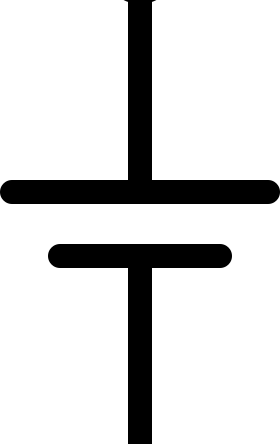
\includegraphics[scale=0.125]{BatterySymbol.png} & Battery & A battery is represented by a long line and a short line stacked on top of each other.  Sometimes, there are two sets of long and short lines.  The long line is the positive terminal and the short line is the negative terminal (which is usually used as the ground). \\ \hline
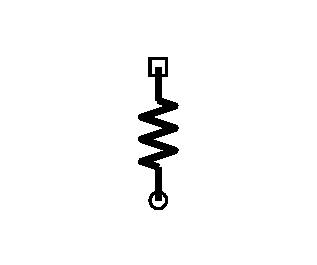
\includegraphics[scale=0.25]{ResistorSymbol.pdf} & Resistor & A resistor is represented by a sharp, wavy line with wires coming out of each side. \\ \hline
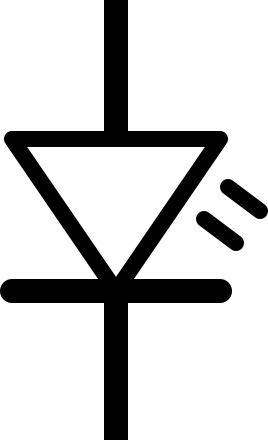
\includegraphics[scale=0.125]{LEDSymbol.png} & LED & An LED is represented by an arrow with a line across it, indicating that current can flow from positive to negative in the direction of the arrow, but it is blocked going the other way.  The LED symbol also has two short lines coming out of it, representing the fact that it emits light. \\
\end{tabular}
\end{center}
\end{figure}

Then, the components are connected together using lines to represent the wires and connections between the components.

Therefore, we can redraw our original circuit using these symbols like you see in Figure~\ref{figCircuitBasicLED}.

\begin{figure}
\caption{Basic LED Circuit Drawn as a Diagram}
\label{figCircuitBasicLED}
\centering
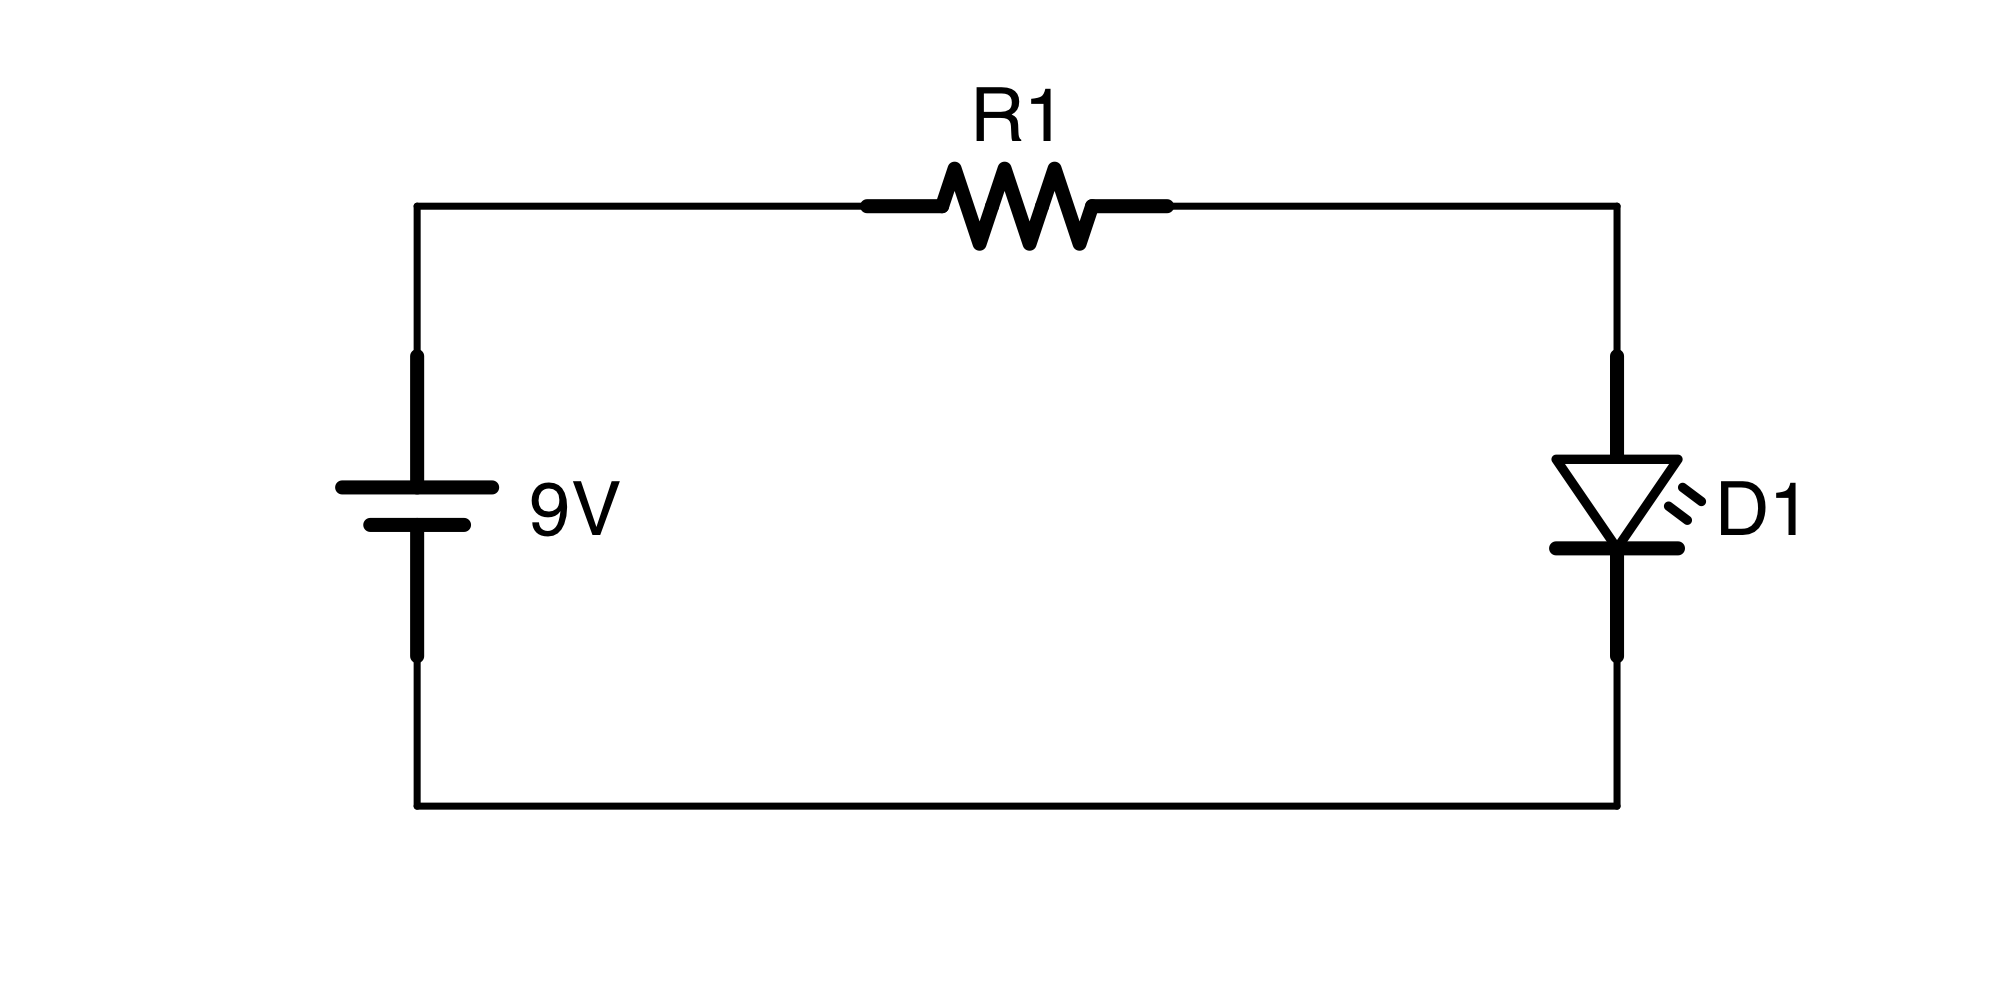
\includegraphics[scale=0.125]{CircuitBasicLED.png}
\end{figure}

Notice that each of our components are laid out on the diagram with wires connecting them.
Remember that it doesn't matter if we have very long wires, very short wires, or if the components are directly placed end-to-end---the resulting circuits will operate identically.
Also notice that each component is labeled (R1 and D1) because, as we make more complicated circuits, it is important to be able to refer back to them.

It does not matter in a diagram which way you have your components turned, how long or short your wires are, or what the general spacing looks like.
When you actually wire it, all of those things will change.
The important part of a circuit diagram is to convey to the reader what the parts are, how they are connected, and what the circuit does in the way that is easiest to read.

For instance, all of the circuits in Figure~\ref{figCircuitLEDAlt} are equivalent to the circuit in Figure~\ref{figCircuitBasicLED}, they are just drawn differently.

\begin{figure}
\caption{Alternative Ways of Drawing the Basic LED Circuit}
\centering
\label{figCircuitLEDAlt}
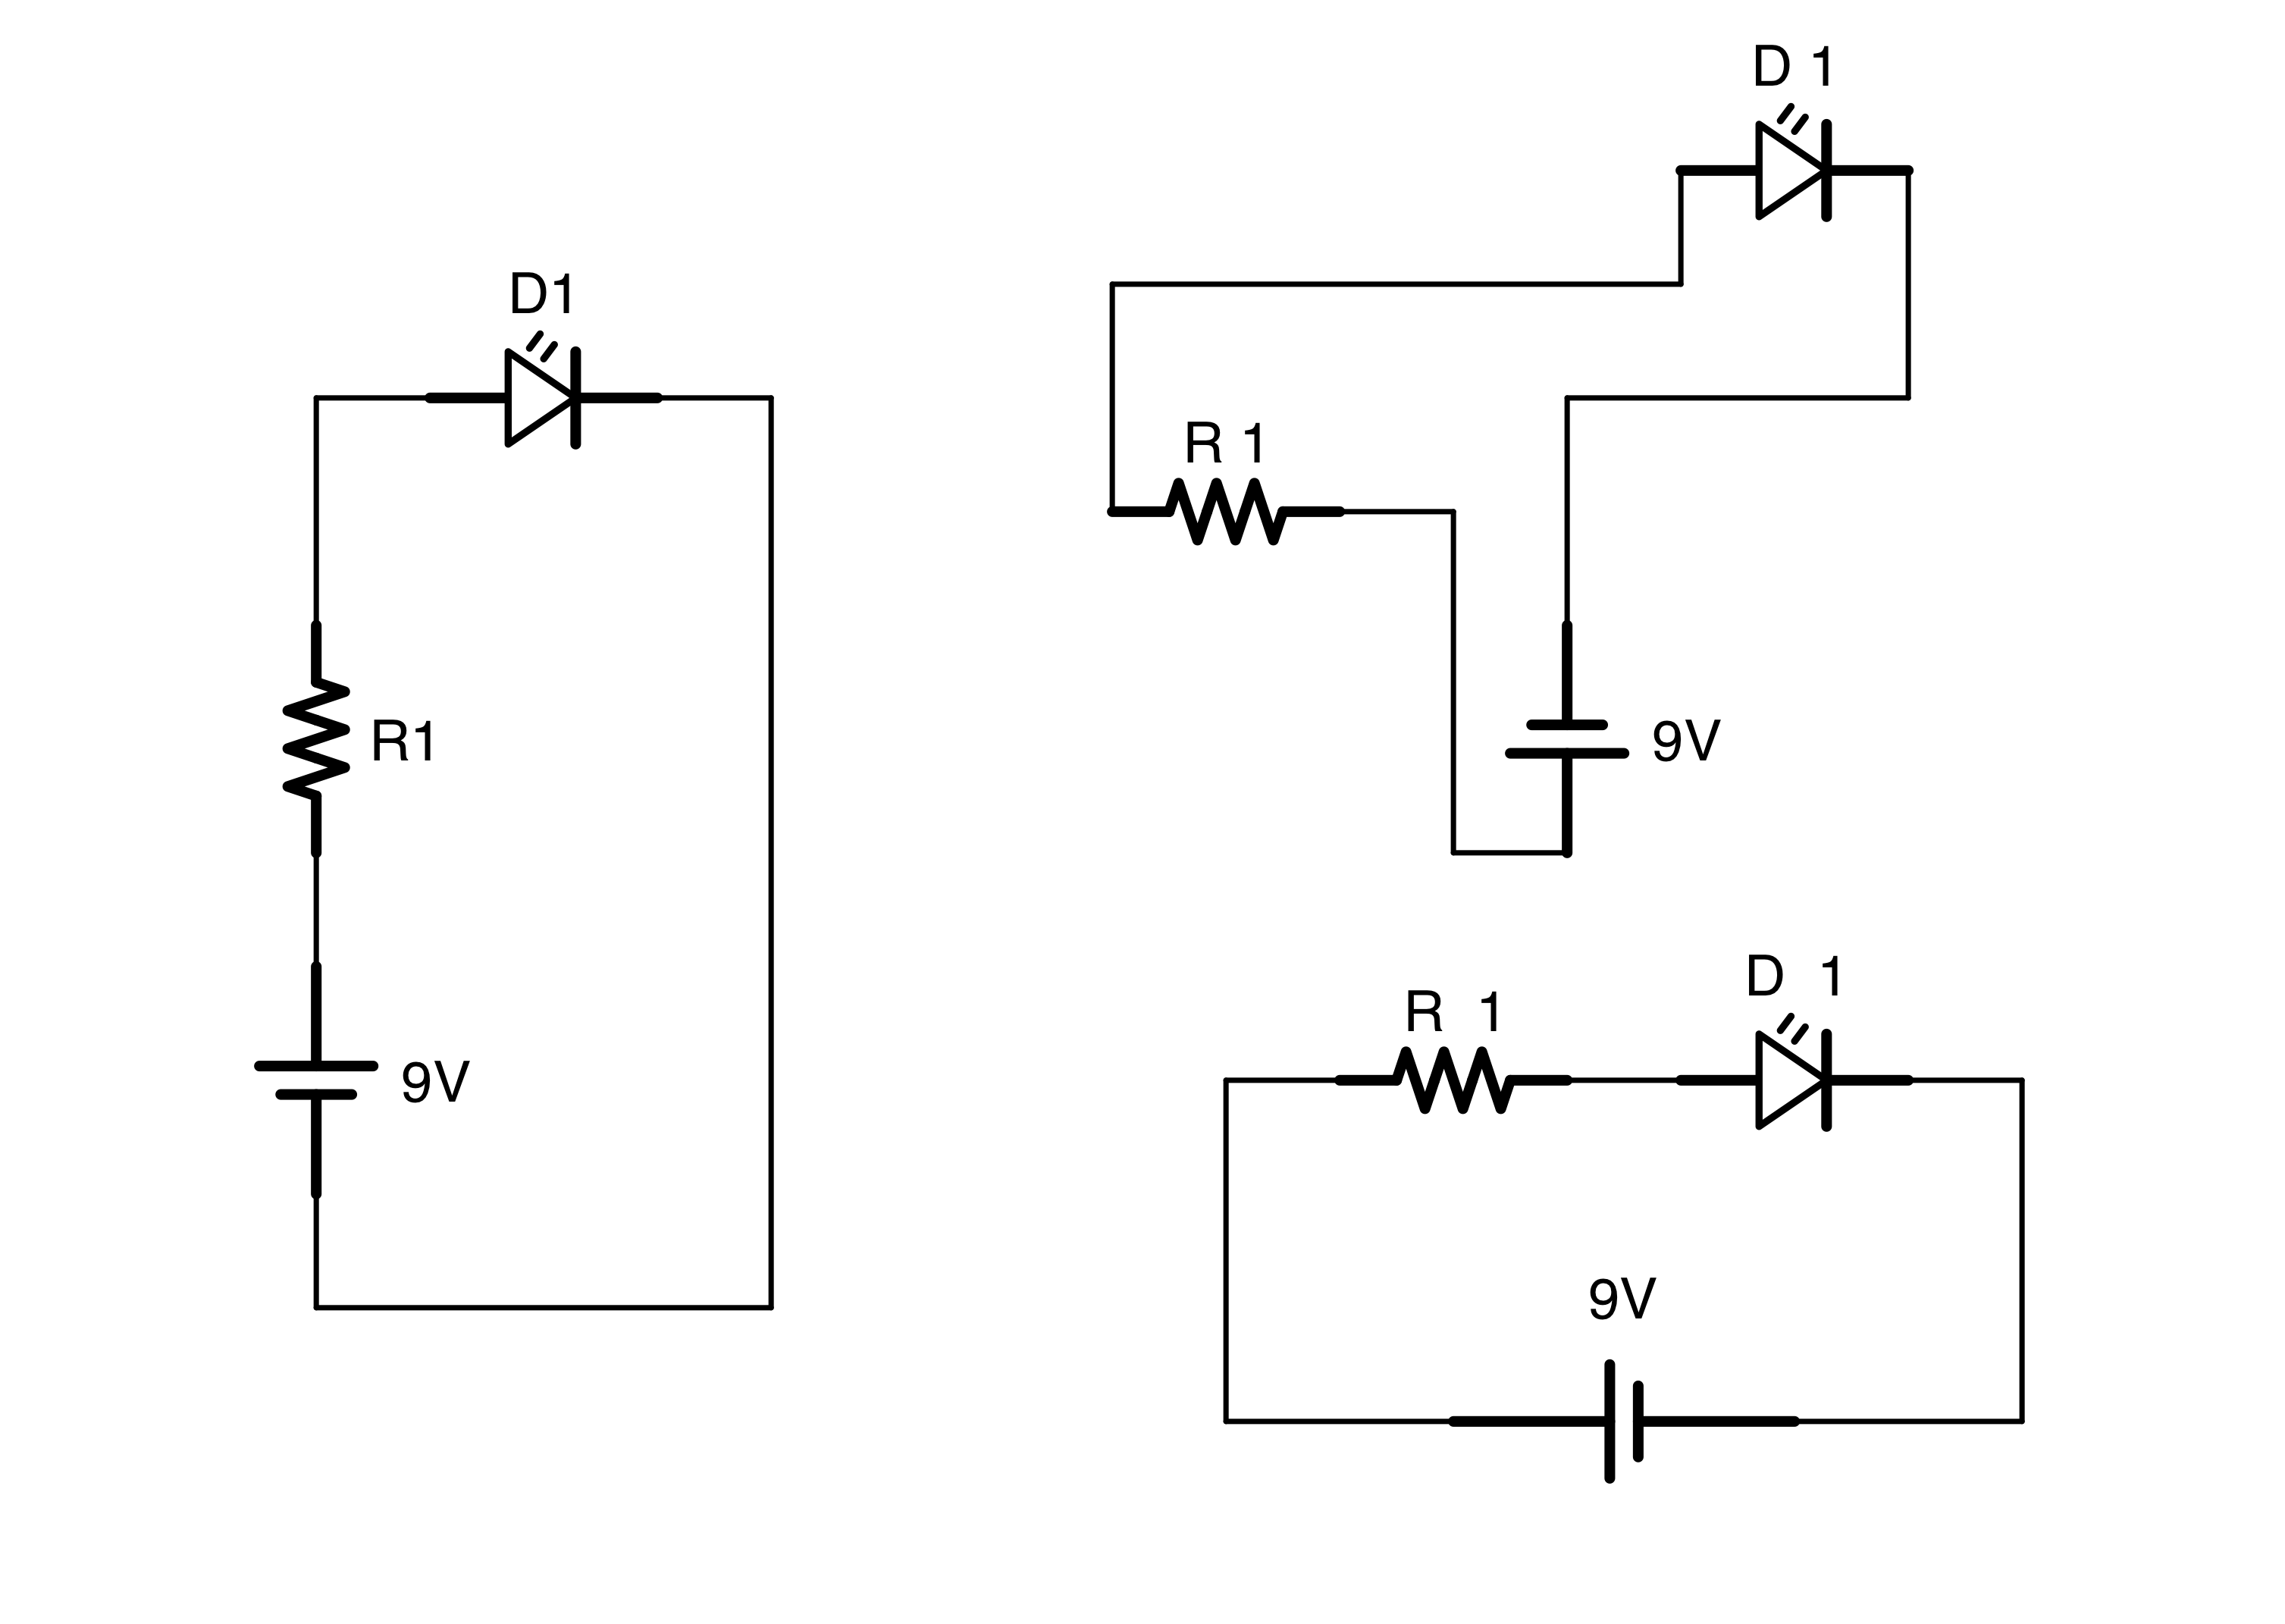
\includegraphics[scale=0.08]{CircuitLEDAlt}
\end{figure}

For consistency, I like to draw all of my batteries to the left of the drawing with the positive side on top.
By keeping the battery positive-side-up, components with higher voltage are usually closer to the top, and components with lower voltages are usually closer to the bottom, with the ground (i.e., zero volts) coming back into the negative terminal.
I also try to make my wire lines as simple as possible in order to make following them easier.

By keeping some amount of consistency, it is easier to look at a drawing and see what it happening.

\section{Drawing the Ground}

Remember that for electricity to move, every circuit must be fully connected from the positive side to the negative side.
That means that in larger circuits there are numerous connections that come from the positive or go back to the ground/negative.
Because of this, a special symbol has been adopted to refer to the ground point in a circuit.
This symbol, the ground symbol, has three lines, each shorter than the next.
Every point on a circuit that has this symbol connected to it is connected to each other (usually they are all connected to the negative side of the battery).

Therefore, the circuit in Figure~\ref{figCircuitBasicLEDGround} is the same circuit as before, just drawn using the ground symbol.
Since every point with the ground symbol are all connected together, using this symbol on both the negative terminal and the negative side of the LED means that they are wired together.

This doesn't help us a lot for this circuit (and, in fact, it makes it a little less easy to read).  
However, in complex circuits, it is much easier to write the ground symbol than trying to have twenty lines drawn back to the negative terminal.

\simplegraphicsfigure{Basic LED Circuit Drawing Using the Ground Symbol}{CircuitBasicLEDGround}{0.08}

Additionally, the same is true with the positive side of the battery.
Many components require a direct connection to a specific voltage to work correctly.
These are usually marked with just a disconnected wire with the end of the wire marking what voltage it requires.
We make less use of that symbol in this book than the ground symbol, but it does come in handy sometimes.

So, using both the voltage source and the ground symbols, we could rewrite the same circuit again in the manner shown in Figure~\ref{figCircuitBasicLEDPosGround}.
This circuit, again, is not \emph{wired} any differently than before.
We are just \emph{drawing} it differently.
For this circuit, it doesn't matter, but in more complex circuits, if we need a specific voltage at a specific location, this symbol tells us to put it there.

\simplegraphicsfigure{Simple LED Circuit Using Positive and Ground Symbols}{CircuitBasicLEDPosGround}{0.08}

\reviewsection

In this chapter, we learned:

\begin{enumerate}
\item Every circuit requires a source of power (usually a battery), wires and components, some amount of resistance, and a complete path back to the negative side of the power source.
\item An open circuit is one that does not connect back to the negative side (and thus does not provide any electricity), and a short circuit is one that connects back to the negative side without any resistance (and thus overwhelms the circuit with current).
\item Batteries supply a fixed voltage between its two terminals.
\item A resistor provides a fixed resistance (measured in ohms) within your circuit.
\item An LED allows current to flow in only one direction, gives off light when current is flowing, but is destroyed when the current goes above 20--30 milliamps.
\item The longer leg of the LED should be on the positive side of the circuit.
\item Wires on a circuit can be almost any length (from zero to a few meters) without changing the functionality of the circuit.
\item A circuit diagram is a way of drawing a circuit so that it is easy to read and understand what the circuit is doing.
\item Each component has its own symbol in a circuit diagram.
\item Every component labeled with the ground symbol is connected together, usually at the negative side of the battery.
\item Voltage sources can be similarly labeled by a wire connected on one side labeled with the voltage that it is supposed to be carrying.
\end{enumerate}

\applysection

\textbf{Special Note} - In the problems below, since we have not yet studied LED operation in-depth, we are ignoring the electrical characteristics of the LED and just focusing on the resistor.  
If you know how to calculate the circuit characteristics using the LED, please ignore it anyway for the purpose of these exercises.

\begin{enumerate}
\item Calculate the amount of current running in the circuit you built in this chapter using Ohm's law.  Since Ohm's law gives the results in amps, convert the value to milliamps.
\item Let's say that the minimum amount of current needed for the LED to be visibly on is 1 milliamp.  What value of resistor would produce this current?
\item Let's say that the maximum amount of current the LED can handle is 30 milliamps.  What value of resistor would produce this current?
\item Draw a circuit diagram of a short circuit.
\item Take the circuit drawing in this chapter, and modify it so that it is an open circuit.
\item Draw a circuit with just a battery and a resistor.  Make up values for both the battery and the resistor and calculate the amount of current flowing through.
\end{enumerate}
